\section{SMC model} \label{sec:smc_model}
After having produced a near optimal trace from the \gls{cora} model, it will be used to update a \gls{smc} model on which other relevant queries can be run.

The \gls{smc} model is equipped with an implementation of \gls{kibam}\cref{sec:kibam}, in order to make a more accurate representation of the battery dis- or recharge. The \gls{smc} model preserves the solar template in order to allow it to charge during periods of insolation.

Where the \gls{cora} model finds a trace, the \gls{smc} model will try and rerun the produced trace. This means the \gls{smc} model will execute tasks in the exact same order as the \gls{cora} model.% As this model implements KiBaM it gives a fairly accurate representation of the energy consumption. 

\Cref{fig:cost_schedule} and \cref{fig:solar_task}, shows the different templates used in the \gls{smc} model. To the left of \cref{fig:cost_schedule} are the energy source. The energy source is responsible for updating the remaining available and bound energy, and in case there are no more available energy, it will synchronise with the scheduler which will then stop running more tasks.
On the right of \cref{fig:cost_schedule} is the scheduler, it awaits a synchronisation from the tasks in order to ensure that they are ready for execution. The scheduler then estimates if running another task will deplete the battery. If this is the case it will transition back to the initial location preparing to run another task. If running another task would not deplete the battery, the task will be run.

\begin{figure}[H]%
	\centering
	\subfloat
	{{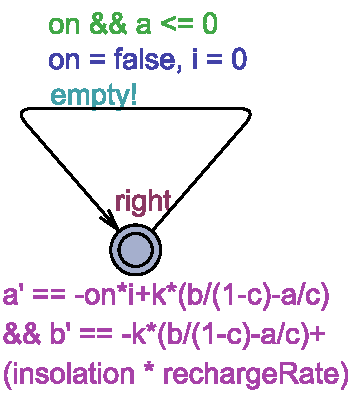
\includegraphics[width=4cm]{graphics/smc_costhandler.pdf} }}%
	\qquad
	\subfloat
	{{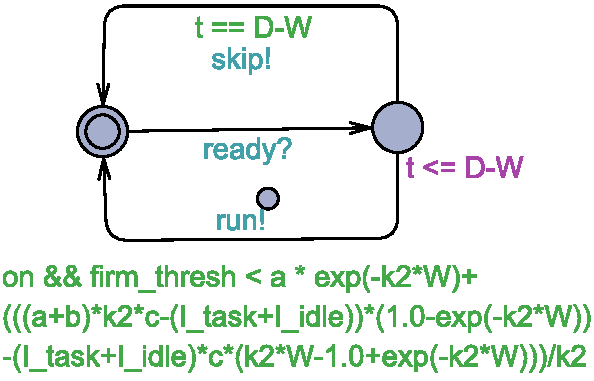
\includegraphics[width=6cm]{graphics/smc_scheduler.pdf} }}%
	\caption{The \gls{smc} model's energy source(left) and scheduler(right)}%
	\label{fig:cost_schedule}%
\end{figure}

On the left side of \cref{fig:solar_task}, we see the template for the orbit time. It is here assumed that the satellite will spend half its orbit in insolation where it is possible to recharge the battery. It switches the variable \uppVar{Insolation} between true and false, which is used in the calculation of the bound energy.\afx{Kom tilbage hertil når at kibam afsnittet er frdigt. Uddyb om hvordan vores mplementation reflektere teorien fra \cref{sec:kibam}}\\
The right side of \cref{fig:solar_task} is the template for a task, this indicates that a task can be, ready to be run, running, and inactive. When a task is not running the consumption is lower as indicated by \uppVar{i = I\_idle} which represents the background load of other minor tasks that are not modelled.

\begin{figure}[H]%
	\centering
	\subfloat
	{{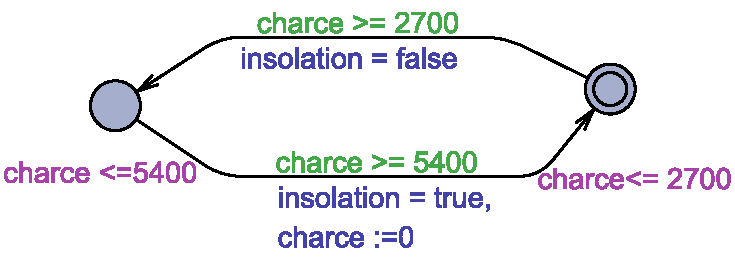
\includegraphics[width=8cm]{graphics/smc_solar.pdf} }}%
	\qquad
	\subfloat
	{{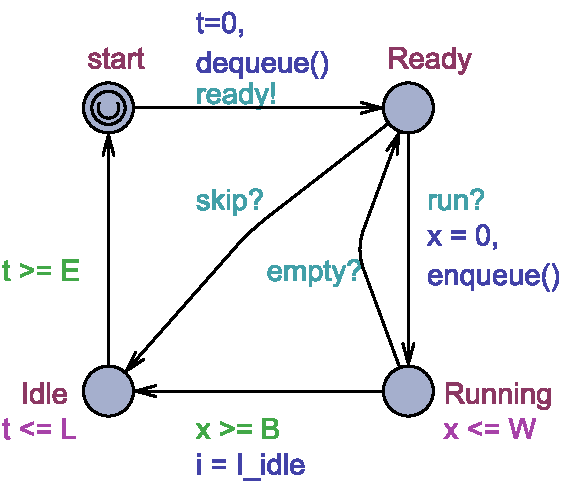
\includegraphics[width=6cm]{graphics/smc_task.pdf} }}%
	\caption{The \gls{smc} model's representation of solar panels(left) and a task(right)}%
	\label{fig:solar_task}%
\end{figure}
Since the model is made in UPPAAL \gls{smc} we are able to run statistical queries asking for the chance of the available energy falling below some threshold, or to simply track the value of the bound and available energy over time for some specified amount of runs. Examples of such queries can be seen in \cref{eq:pr_low_a_sim_ab}, which indicates, first the chance that the battery level will fall below $55\, \%$ within $43200$ time units. Assuming the time unit is in seconds the example query is for 12 hours. The other query is a simulation of the avilable and bound energy over the same amount of time.\\
\begin{align}
Pr[<= 43200] \quad(a <= (c/100)*55)		\nonumber \\
simulate \quad 1 \quad [<=432000] \quad \{a,b\} 
\label{eq:pr_low_a_sim_ab}
\end{align}

The advantages of running these queries is, that even though the runs in \gls{cora} conclude that a schedule is viable, the probability query may be able to find that running the trace could lead to energy depletion. Also tacking the state of the battery may help to see the effect of the solar panels and the tasks stress on the battery. This is relevant as one or two repetitions of the schedule may not deplete the battery but perhaps ten would, in such case it may be relevant to change some parameters and run it again.
\afx{skriv om robustheden også}



\subsection*{Templates}
\subsubsection*{Processor}
\begin{figure}
	\centering
	\begin{tikzpicture}
	%Locations
	\node [init] (l0) {$\cup$};
	\node [location] (l1) [right of=l0, xshift=40mm, label={
		[align=left]above:
		\textcolor{name}{PrepNext}},
		label={
		[align=center]below:
		\textcolor{invariant}{totalTime <= RunStart[payloadNumber]}
	}] {};
	\node [location] (l2) [right of=l1, xshift=80mm, label={
		[align=left]above:
		\textcolor{name}{Ready}
	}] {};
	\node [location] (l3) [below of=l0, yshift=-40mm, label={
		[align=left]below:
		\textcolor{name}{Done}
	}] {};
	\node [location] (l4) [below of=l1, yshift=-40mm, label={
		[align=left]below:
		\textcolor{name}{Idle}\\
		\textcolor{invariant}{x <= D}
	}] {};
	\node [location] (l5) [below of=l2, yshift=-40mm, label={
		[align=left]below:
		\textcolor{name}{Running}\\
		\textcolor{invariant}{x <= W}
	}] {};
	\path[->,black] (l0) edge node [midway, above][align=left]{
		\textcolor{update}{t=0,i = IIdle,}\\
		\textcolor{update}{setActive()}} (l1);
	\path[->,black] (l1) edge node [midway, above][align=center]{
		\textcolor{guard}{totalTime >=RunStart[payloadNumber]}\\
		\textcolor{sync}{ready!}\\
		\textcolor{update}{x=0, t=0,}\\
		\textcolor{update}{dequeue()}} (l2);
	\path[->,black] (l2) edge node [midway, left][align=left]{
		\textcolor{sync}{run?}\\
		\textcolor{update}{x := 0,}\\
		\textcolor{update}{setActive(),}\\
		\textcolor{update}{enqueue()}} (l5);
	\path[->,black] (l5) edge[bend right=45] node [midway, right][align=left]{
		\textcolor{sync}{empty?}} (l2);
	\path[->,black] (l4) edge node [midway, left][align=left]{
		\textcolor{sync}{skip?}\\
		\textcolor{update}{payloadNumber ++,}\\
		\textcolor{update}{skipped()}} (l2);
	\path[->,black] (l5) edge node [midway, below][align=left]{
		\textcolor{guard}{x >= B}\\
		\textcolor{update}{i = IIdle, active = -1,}\\
		\textcolor{update}{payloadNumber ++}} (l4);
	\path[->,black] (l4) edge node [midway, left][align=left]{
		\textcolor{guard}{x >= D \&\&}\\
		\textcolor{guard}{!done()}\\
		\textcolor{update}{setActive()}} (l1);
	\path[->,black] (l4) edge node [midway, below][align=left]{
		\textcolor{guard}{done()}\\
		\textcolor{update}{on = false,}\\
		\textcolor{update}{active = -1}} (l3);
	\end{tikzpicture}
	\caption{Processor template}
	\label{fig:smc_P}
\end{figure}

\subsubsection*{Insolation}
\begin{figure}
	\centering
	\begin{tikzpicture}
	%Locations
	\node [init] (l0) [label={
		[align=left]left:
		\textcolor{invariant}{charge<= OrbitTime/2}
		}] {};
	\node [location] (l1) [right of=l0, xshift=40mm, label={
		[align=left]right:
		\textcolor{invariant}{charge <=OrbitTime}
		}] {};
	\path[->,black] (l0) edge[bend left=45] node [midway, above][align=left]{
		\textcolor{guard}{charge >= OrbitTime/2}\\
		\textcolor{update}{insolation = false}} (l1);
	\path[->,black] (l1) edge[bend left=45] node [midway, below][align=left]{
		\textcolor{guard}{charge >= OrbitTime}\\
		\textcolor{update}{insolation = true,}\\
		\textcolor{update}{charge :=0}} (l0);
	\end{tikzpicture}
	\caption{Insolation template}
	\label{fig:smc_I}
\end{figure}

\subsubsection*{EnergySource}
\begin{figure}
	\centering
	\begin{tikzpicture}
	%Locations
	\node [init] (l0) [label={
		[align=left]left:
		\textcolor{invariant}{a' == -on*i+k*(b/(1-c)-a/c)}\\
		\textcolor{invariant}{\&\& b' == -k*(b/(1-c)-a/c)}\\
		\textcolor{invariant}{+(insolation * RechargeRate)}
	}] {};
	\node [location] (l1) [right of=l0, xshift=40mm, label={
		[align=left]right:
		\textcolor{invariant}{a' == -on*i+k*(b/(1-c)-a/c)}\\
		\textcolor{invariant}{\&\& b' == -k*(b/(1-c)-a/c)}
	}] {};
	\path[->,black] (l0) edge node [midway, above][align=left]{
		\textcolor{guard}{b > MaxB}\\
		\textcolor{sync}{capacityFull!}} (l1);
	\path[->,black] (l1) edge[bend left=45] node [midway, below][align=left]{
		\textcolor{guard}{b < c\_C}\\
		\textcolor{sync}{capacityFull!}} (l0);
	\path[->,black] (l1) edge[loop above] node [midway, above][align=left]{
		\textcolor{guard}{on \&\& a <= 0}\\
		\textcolor{sync}{empty!}\\
		\textcolor{update}{on = false, i = 0}} (l1);
	\path[->,black] (l0) edge[loop above] node [midway, above][align=left]{
		\textcolor{guard}{on \&\& a <= 0}\\
		\textcolor{sync}{empty!}\\
		\textcolor{update}{on = false, i = 0}} (l0);
	\end{tikzpicture}
	\caption{EnergySource template}
	\label{fig:smc_ES}
\end{figure}

\subsubsection*{Scheduler}
\begin{figure}
	\centering
	\begin{tikzpicture}
	%Locations
	\node [init] (l0) {};
	\node [location] (l1) [below of=l0, yshift=-40mm, label={
		[align=left]below:
		\textcolor{invariant}{t <= Payloads[Queue[payloadNumber]][2] - }\\
		\textcolor{invariant}{Payloads[Queue[payloadNumber]][1]}
	}] {};
	\path[->,black] (l1) edge[bend left=50] node [midway, left][align=left]{
		\textcolor{guard}{t == Payloads[Queue[payloadNumber]][2] - }\\
		\textcolor{guard}{Payloads[Queue[payloadNumber]][1]}\\
		\textcolor{sync}{skip!}
	} (l0);
	\path[->,black] (l0) edge node [midway, left][align=left]{
		\textcolor{sync}{ready?}} (l1);
	\path[->,black] (l1) edge[bend right=45] node [midway, right][align=left]{
		\textcolor{guard}{on \&\& mayRun() \&\&}\\
		\textcolor{guard}{FirmThreshold < a * exp(-k2*W)+}\\
		\textcolor{guard}{(((a+b)*k2*c-(IPayload+IIdle))*(1.0-exp(-k2*W))}\\
		\textcolor{guard}{-(IPayload+IIdle)*c*(k2*W-1.0+exp(-k2*W)))/k2}\\
		\textcolor{sync}{run!}\\
		\textcolor{update}{runs[active] ++,}\\
		\textcolor{update}{totalRuns[active] ++}
	} (l0);
	\end{tikzpicture}
	\caption{Task template}
	\label{fig:cora_inso}
\end{figure}

\subsubsection*{OrbitWindows}
\begin{figure}
	\centering
	\begin{tikzpicture}
	%Locations
	\node [init] (l0) [label={
		[align=left]left:
		\textcolor{invariant}{wtime <= Window[id][0]}}] {};
	\node [location] (l1) [right of=l0, xshift=40mm, label={
		[align=left]right:
		\textcolor{invariant}{wtime <= Window[id][1]}
	}] {};
	\node [location] (l2) [below of=l0, xshift=25mm, yshift=-40mm, label={
		[align=left]below:
		\textcolor{invariant}{wtime <= OrbitTime}
	}] {};
	\path[->,black] (l0) edge node [midway, above][align=left]{
		\textcolor{guard}{wtime >= Window[id][0]}\\
		\textcolor{update}{setRunnable(),}\\
		\textcolor{update}{inWindow[id] = 1}
	} (l1);
	\path[->,black] (l1) edge node [midway, right][align=left]{
		\textcolor{guard}{wtime >= Window[id][1]}\\
		\textcolor{update}{setRunnable(),}\\
		\textcolor{update}{inWindow[id] = 0}
	} (l2);
	\path[->,black] (l2) edge node [midway, left][align=left]{
		\textcolor{guard}{wtime >= OrbitTime}\\
		\textcolor{update}{wtime = 0}
	} (l0);
	\end{tikzpicture}
	\caption{OrbitWindows template}
	\label{fig:smc_OW}
\end{figure}
